% Week 9: Decoding Strategies
% BSc Discovery Two-Tier: 20 main + 15 appendix
% Quality-diversity tradeoff hook

% Master Template for NLP Course
% Optimal Readability Layout Standard
% All presentations should include this template

\documentclass[8pt,aspectratio=169]{beamer}
\usetheme{Madrid}
\setbeamertemplate{navigation symbols}{}

% ====================================
% OPTIMAL READABILITY COLOR PALETTE
% ====================================
\definecolor{PureBlack}{HTML}{000000}      % Main text (21:1 contrast)
\definecolor{DeepBlue}{HTML}{003D7A}       % Primary accent (12.6:1 contrast)
\definecolor{DarkGray}{HTML}{4A4A4A}       % Secondary text (9.7:1 contrast)
\definecolor{LightGray}{HTML}{E5E5E5}      % Borders and grids
\definecolor{ChartBlue}{HTML}{0066CC}      % Chart primary
\definecolor{ChartOrange}{HTML}{FF8800}    % Chart secondary
\definecolor{ChartTeal}{HTML}{00A0A0}      % Chart tertiary
\definecolor{ChartPurple}{HTML}{8B4789}    % Chart quaternary
\definecolor{DarkGreen}{HTML}{228B22}      % Success/positive
\definecolor{DarkRed}{HTML}{CC0000}        % Warning/negative

% ====================================
% BEAMER COLOR CONFIGURATION
% ====================================
\setbeamercolor{structure}{fg=PureBlack}
\setbeamercolor{frametitle}{fg=PureBlack,bg=white}
\setbeamercolor{title}{fg=PureBlack,bg=white}
\setbeamercolor{subtitle}{fg=DarkGray}
\setbeamercolor{author}{fg=DarkGray}
\setbeamercolor{date}{fg=DarkGray}
\setbeamercolor{institute}{fg=DarkGray}

% Blocks - no backgrounds
\setbeamercolor{block title}{fg=PureBlack,bg=white}
\setbeamercolor{block body}{fg=PureBlack,bg=white}
\setbeamercolor{block title example}{fg=DarkGreen,bg=white}
\setbeamercolor{block body example}{fg=PureBlack,bg=white}
\setbeamercolor{block title alerted}{fg=DarkRed,bg=white}
\setbeamercolor{block body alerted}{fg=PureBlack,bg=white}

% Lists
\setbeamercolor{item}{fg=DeepBlue}
\setbeamercolor{subitem}{fg=ChartBlue}
\setbeamercolor{enumerate item}{fg=DeepBlue}
\setbeamercolor{enumerate subitem}{fg=ChartBlue}

% Text
\setbeamercolor{normal text}{fg=PureBlack,bg=white}
\setbeamercolor{alerted text}{fg=DarkRed}
\setbeamercolor{example text}{fg=DarkGreen}

% Footer
\setbeamercolor{footline}{fg=DarkGray,bg=white}
\setbeamercolor{page number in head/foot}{fg=DarkGray}

% ====================================
% FONT CONFIGURATION
% ====================================
\setbeamerfont{normal text}{size=\normalsize}
\setbeamerfont{frametitle}{size=\Large,series=\bfseries}
\setbeamerfont{title}{size=\huge,series=\bfseries}
\setbeamerfont{subtitle}{size=\large}
\setbeamerfont{author}{size=\normalsize}
\setbeamerfont{date}{size=\small}
\setbeamerfont{institute}{size=\small}

% ====================================
% REQUIRED PACKAGES
% ====================================
\usepackage{tikz}
\usepackage{amsmath}
\usepackage{amssymb}
\usepackage{booktabs}
\usepackage{graphicx}
\usepackage{array}
\usepackage{listings}
\usepackage{algorithm2e}
\usepackage{xcolor}
\usepackage{tabularx}
\usepackage{multirow}
\usepackage{subcaption}

% ====================================
% CUSTOM COMMANDS
% ====================================
% Text highlighting commands
\newcommand{\highlight}[1]{\textcolor{DeepBlue}{\textbf{#1}}}
\newcommand{\secondary}[1]{\textcolor{DarkGray}{#1}}
\newcommand{\success}[1]{\textcolor{DarkGreen}{#1}}
\newcommand{\warning}[1]{\textcolor{DarkRed}{#1}}
\newcommand{\data}[1]{\textcolor{ChartBlue}{#1}}
\newcommand{\dataalt}[1]{\textcolor{ChartOrange}{#1}}

% Mathematical notation
\newcommand{\given}{\mid}
\newcommand{\prob}[1]{P(#1)}
\newcommand{\argmax}{\operatorname*{argmax}}
\newcommand{\argmin}{\operatorname*{argmin}}
\newcommand{\softmax}{\operatorname{softmax}}

% Box commands for emphasis
\newcommand{\keypoint}[1]{%
  \begin{center}
  \fbox{\parbox{0.9\textwidth}{\centering\textbf{#1}}}
  \end{center}
}

\newcommand{\formula}[1]{%
  \begin{center}
  \colorbox{LightGray}{\parbox{0.8\textwidth}{\centering$\displaystyle #1$}}
  \end{center}
}

% ====================================
% LISTINGS CONFIGURATION
% ====================================
\lstset{
  basicstyle=\ttfamily\small,
  keywordstyle=\color{DeepBlue}\bfseries,
  commentstyle=\color{DarkGray}\itshape,
  stringstyle=\color{ChartOrange},
  numbers=left,
  numberstyle=\tiny\color{DarkGray},
  stepnumber=1,
  numbersep=5pt,
  backgroundcolor=\color{white},
  showspaces=false,
  showstringspaces=false,
  showtabs=false,
  frame=single,
  frameround=tttt,
  rulecolor=\color{LightGray},
  tabsize=2,
  captionpos=b,
  breaklines=true,
  breakatwhitespace=true,
  language=Python,
  escapeinside={(*@}{@*)},
  morekeywords={self, yield, assert, with, as}
}

% ====================================
% STANDARD SLIDE LAYOUTS
% ====================================

% Two-column layout with title
\newcommand{\twocolslide}[3]{%
  \begin{frame}{#1}
  \begin{columns}[T]
  \column{0.48\textwidth}
  #2
  \column{0.48\textwidth}
  #3
  \end{columns}
  \end{frame}
}

% Three-column layout
\newcommand{\threecolslide}[4]{%
  \begin{frame}{#1}
  \begin{columns}[T]
  \column{0.32\textwidth}
  #2
  \column{0.32\textwidth}
  #3
  \column{0.32\textwidth}
  #4
  \end{columns}
  \end{frame}
}

% Chart slide with caption
\newcommand{\chartslide}[3]{%
  \begin{frame}{#1}
  \begin{center}
  \includegraphics[width=#2\textwidth]{#3}
  \end{center}
  \end{frame}
}

% Full chart slide - optimized to 0.85 for proper margins
\newcommand{\fullchartslide}[2]{%
  \begin{frame}{#1}
  \begin{center}
  \includegraphics[width=0.85\textwidth]{#2}
  \end{center}
  \end{frame}
}

% Code slide
\newcommand{\codeslide}[3]{%
  \begin{frame}[fragile]{#1}
  \begin{lstlisting}[language=#2]
#3
  \end{lstlisting}
  \end{frame}
}

% Concept slide with figure
\newcommand{\conceptslide}[3]{%
  \begin{frame}{#1}
  \begin{columns}[T]
  \column{0.6\textwidth}
  #2
  \column{0.35\textwidth}
  \begin{center}
  \includegraphics[width=0.95\textwidth]{#3}
  \end{center}
  \end{columns}
  \end{frame}
}

% Table slide
\newcommand{\tableslide}[2]{%
  \begin{frame}{#1}
  \begin{center}
  \Large
  \renewcommand{\arraystretch}{1.5}
  #2
  \end{center}
  \end{frame}
}

% Summary slide
\newcommand{\summaryslide}[2]{%
  \begin{frame}{#1}
  \begin{center}
  \Large
  #2
  \end{center}
  \vfill
  \begin{center}
  \keypoint{Key Takeaway}
  \end{center}
  \end{frame}
}

% ====================================
% REMOVE DECORATIONS
% ====================================
\setbeamertemplate{blocks}[default]
\setbeamertemplate{title page}[default][colsep=-4bp,rounded=false]
\setbeamertemplate{itemize items}[circle]
\setbeamertemplate{enumerate items}[default]
\setbeamertemplate{section in toc}[sections numbered]
\setbeamertemplate{subsection in toc}[subsections numbered]

% ====================================
% PAGE NUMBERING
% ====================================
\setbeamertemplate{footline}{
  \leavevmode%
  \hbox{%
  \begin{beamercolorbox}[wd=.333333\paperwidth,ht=2.25ex,dp=1ex,center]{author in head/foot}%
    \usebeamerfont{author in head/foot}\secondary{\insertshortauthor}
  \end{beamercolorbox}%
  \begin{beamercolorbox}[wd=.333333\paperwidth,ht=2.25ex,dp=1ex,center]{title in head/foot}%
    \usebeamerfont{title in head/foot}\secondary{\insertshorttitle}
  \end{beamercolorbox}%
  \begin{beamercolorbox}[wd=.333333\paperwidth,ht=2.25ex,dp=1ex,right]{date in head/foot}%
    \usebeamerfont{date in head/foot}\secondary{\insertshortdate{}\hspace*{2em}
    \insertframenumber{} / \inserttotalframenumber\hspace*{2ex}}
  \end{beamercolorbox}}%
  \vskip0pt%
}

% ====================================
% TABLE OF CONTENTS STYLE
% ====================================
\setbeamertemplate{section in toc}{%
  \leavevmode\leftskip=1.5em%
  \llap{%
    \usebeamerfont{section in toc}%
    \usebeamercolor[fg]{section in toc}%
    \inserttocsectionnumber.%
  }%
  \usebeamerfont{section in toc}%
  \usebeamercolor[fg]{section in toc}%
  \inserttocsection\par%
}

\setbeamertemplate{subsection in toc}{%
  \leavevmode\leftskip=3em%
  \llap{%
    \usebeamerfont{subsection in toc}%
    \usebeamercolor[fg]{subsection in toc}%
    \inserttocsectionnumber.\inserttocsubsectionnumber%
  }%
  \usebeamerfont{subsection in toc}%
  \usebeamercolor[fg]{subsection in toc}%
  \inserttocsubsection\par%
}

% ====================================
% END OF MASTER TEMPLATE
% ====================================

\newcommand{\bottomnote}[1]{\vspace{0.2cm}\begin{center}\footnotesize\secondary{#1}\end{center}}

\title{Decoding Strategies}
\subtitle{\secondary{Week 9 - From Greedy to Creative}}
\author{NLP Course 2025}
\date{October 27, 2025}

\begin{document}

% MAIN (20 SLIDES)

\begin{frame}
\titlepage
\vfill
\begin{center}\secondary{\footnotesize Two-Tier BSc Discovery}\end{center}
\end{frame}

% Hook (2)
\begin{frame}[t]{The Quality-Diversity Tradeoff}
\vspace{-0.3cm}
\begin{center}
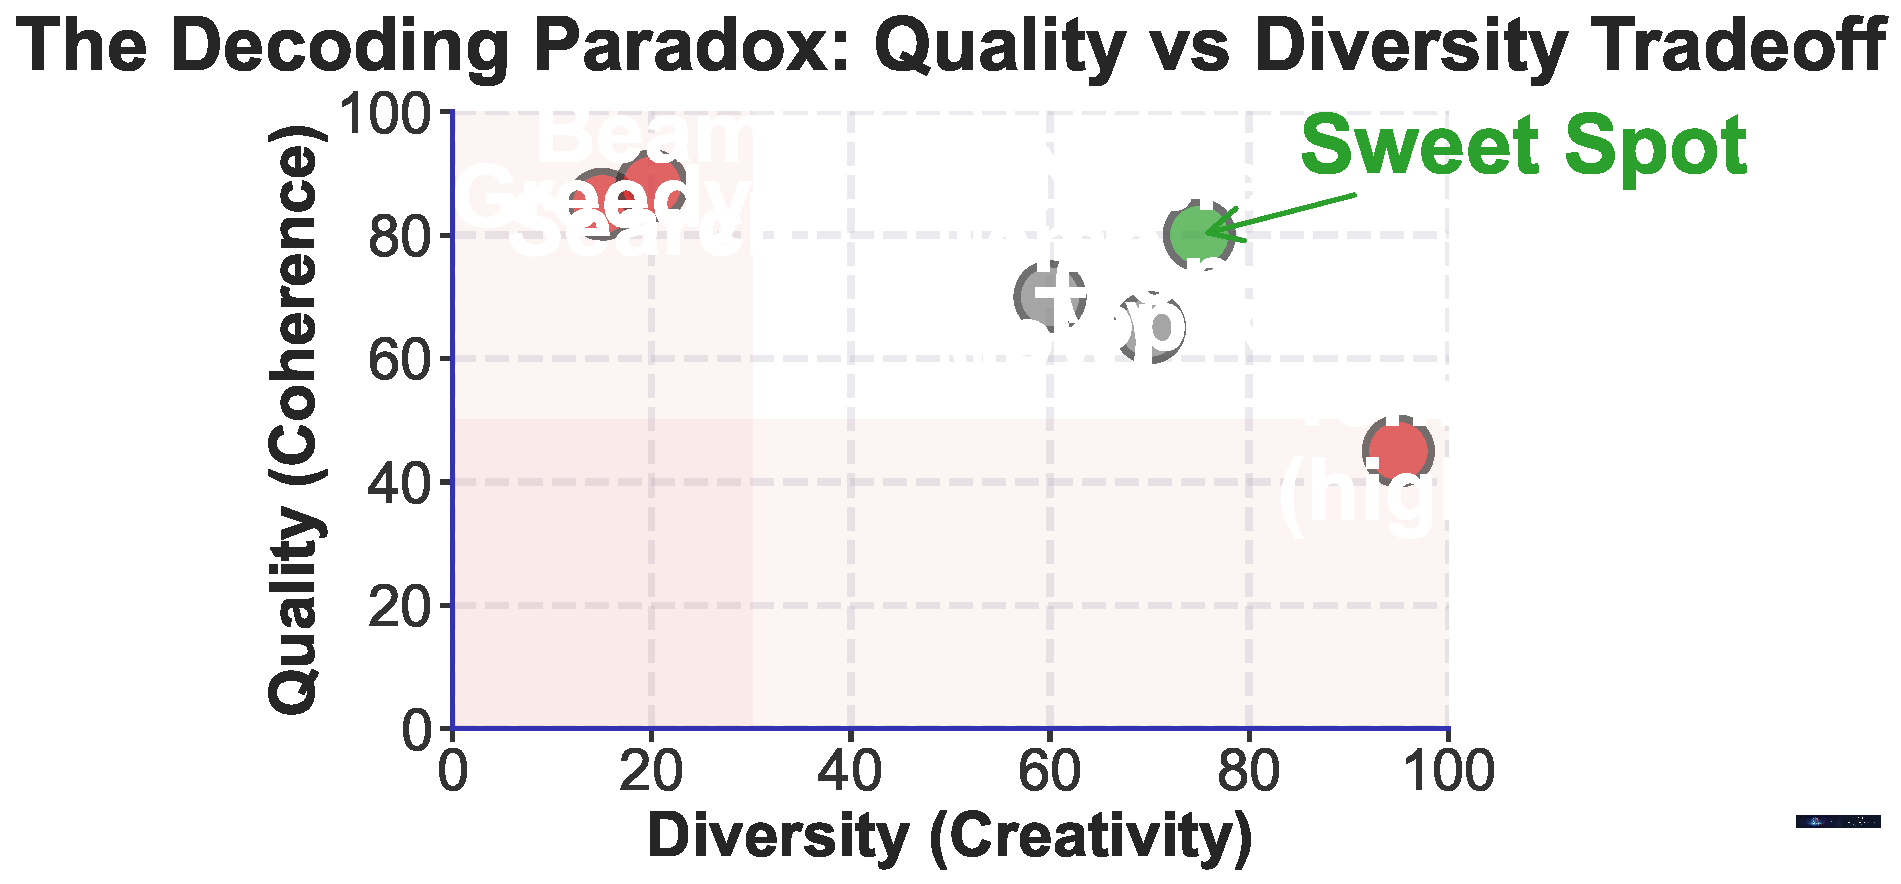
\includegraphics[width=0.7\textwidth]{../figures/quality_diversity_tradeoff_bsc.pdf}
\end{center}
\begin{center}
\textbf{Key Insight}: Best text is boring, creative text is nonsense - need balance
\end{center}
\bottomnote{Greedy: deterministic and dull. Random: diverse but incoherent.}
\end{frame}

\begin{frame}[t]{Three Decoding Families}
\small
\begin{columns}[T]
\column{0.32\textwidth}
\textbf{Deterministic}

Greedy, Beam

Always same output

High quality

No diversity

\column{0.32\textwidth}
\textbf{Stochastic}

Temperature, Top-k

Random sampling

Creative

Can be nonsense

\column{0.32\textwidth}
\textbf{Controlled}

Nucleus (top-p)

Balance both

Tunable creativity

Modern standard
\end{columns}
\bottomnote{Different tasks need different decoding strategies}
\end{frame}

% Greedy/Beam (6: slides 4-9)
\begin{frame}[t]{Beam Search: Explore Multiple Paths}
\vspace{-0.3cm}
\begin{center}
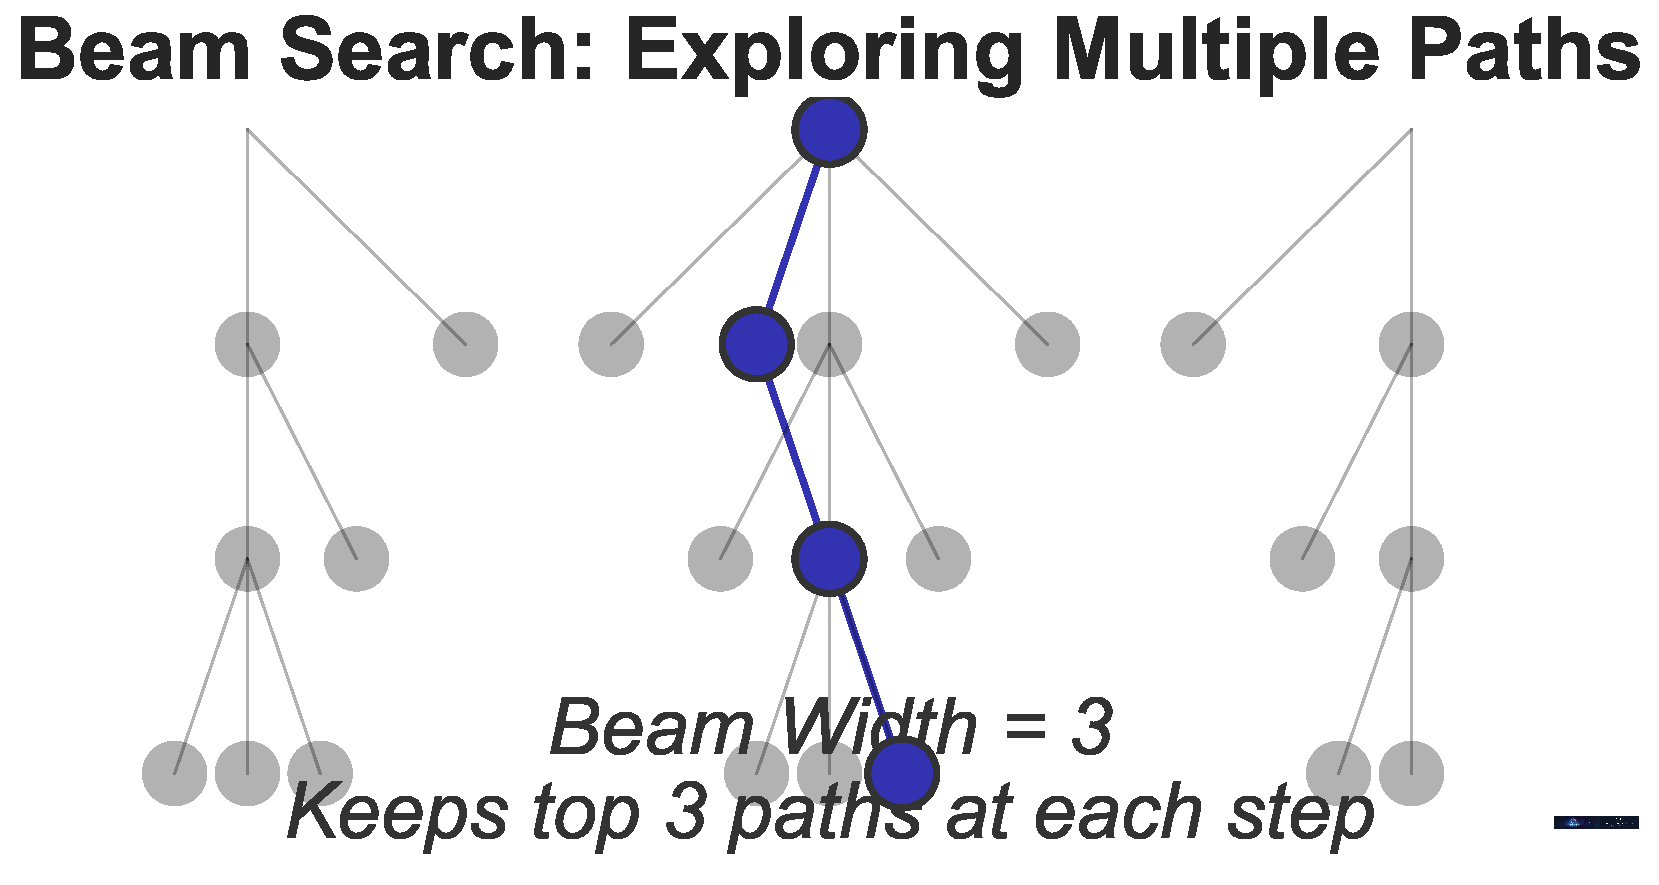
\includegraphics[width=0.7\textwidth]{../figures/beam_search_visual_bsc.pdf}
\end{center}
\begin{center}
\textbf{Key Insight}: Keep top-k hypotheses at each step - find better sequences
\end{center}
\bottomnote{Beam width = 5 typical. Balance between greedy (1) and exhaustive (∞)}
\end{frame}

\begin{frame}[t]{Worked Example: Beam Search (width=3)}
\small
\textbf{Task}: Generate after ``The cat''

\vspace{3mm}
\textbf{Step 1}: Top-3 words

sat (0.4), is (0.3), was (0.2)

Keep 3 hypotheses

\vspace{3mm}
\textbf{Step 2}: Expand each

``The cat sat'' → on (0.5), there (0.3)

``The cat is'' → sleeping (0.6), black (0.2)

``The cat was'' → happy (0.4), tired (0.3)

\vspace{3mm}
\textbf{Step 3}: Score and prune

Total scores: sat+on (0.2), is+sleeping (0.18), sat+there (0.12)

Keep top-3, continue...

\vspace{3mm}
Final: ``The cat is sleeping'' wins!

\bottomnote{Beam search finds better sequences than greedy}
\end{frame}

% Sampling (8: slides 10-17)
\begin{frame}[t]{Temperature: Control Randomness}
\vspace{-0.3cm}
\begin{center}
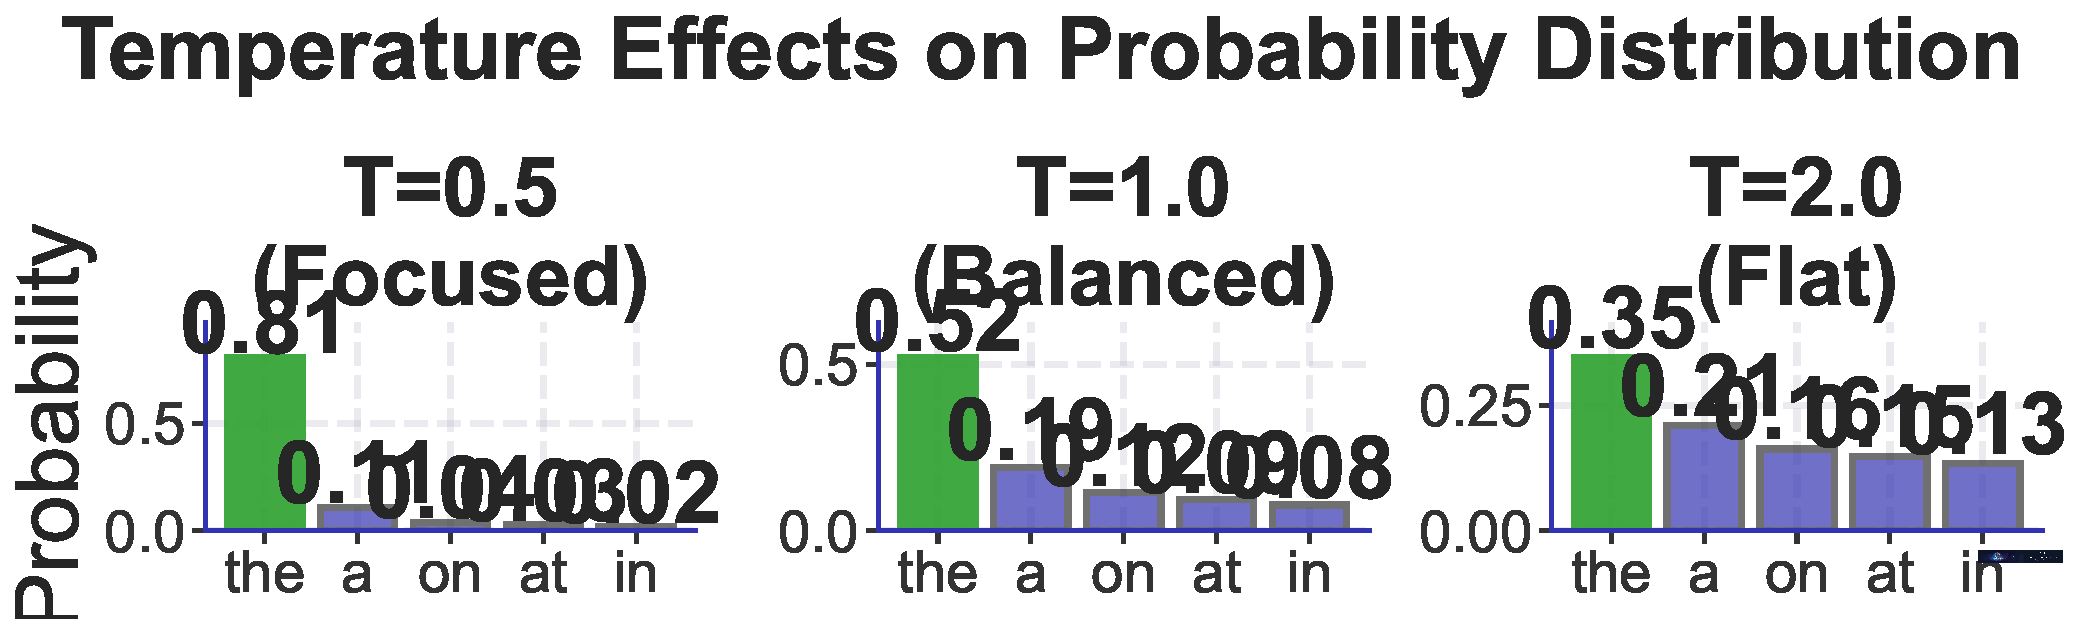
\includegraphics[width=0.65\textwidth]{../figures/temperature_effects_bsc.pdf}
\end{center}
\begin{center}
\textbf{Key Insight}: Temperature controls peakedness of probability distribution
\end{center}
\bottomnote{T=0.5: focused. T=1.0: unchanged. T=2.0: flattened (more random)}
\end{frame}

\begin{frame}[t]{Worked Example: Temperature Scaling}
\small
\textbf{Logits}: [2.0, 1.0, 0.5, 0.2]

\vspace{5mm}
\textbf{T=0.5} (focused):

$$p_i = \frac{\exp(logit_i / 0.5)}{\sum \exp(logit_j / 0.5)}$$

Result: [0.61, 0.22, 0.11, 0.06] - peaked!

\vspace{5mm}
\textbf{T=1.0} (normal):

$$p_i = \softmax(logits)$$

Result: [0.42, 0.23, 0.16, 0.13] - balanced

\vspace{5mm}
\textbf{T=2.0} (flat):

Result: [0.32, 0.26, 0.23, 0.19] - uniform!

\bottomnote{Lower T = more deterministic. Higher T = more random.}
\end{frame}

% Remaining sampling slides...

% Comparison (4: slides 18-20 + summary)
\begin{frame}[t]{Key Takeaways}
\begin{enumerate}
\item Beam search: Deterministic, high quality, no diversity
\item Temperature: Simple randomness control
\item Top-k: Filter unlikely words, sample from top
\item Nucleus (top-p): Dynamic cutoff, modern standard
\item Choose based on task: translation=beam, creative=sampling
\end{enumerate}
\bottomnote{Decoding strategy matters as much as model quality}
\end{frame}

% APPENDIX (15 slides)

\begin{frame}[t]{}
\begin{center}\Huge\textbf{Technical Appendix}\end{center}
\end{frame}

% A1-A5: Beam search mathematics
% A6-A10: Sampling mathematics
% A11-A15: Advanced (constrained, contrastive, quality metrics)

\end{document}
